\section{Autoencoders and Adversarial Examples}\label{sec:combining}
TODO

\subsection{Adversarial Images for Autoencoder}
This approach \cite{smth} describes a method for creating a distortion based
on variational autoencoders: Our attack consists of selecting an original image
and a target image and then feeding the network with the original image added to
a small distortion, optimized to get the result as close as possible to the
target image (Figure \ref{fig:adversarial_images_autoencoder}). Autoencoders
reconstruct from the latent representation, which makes it the information
bottleneck, and therefore particularly convenient to attack. The authors used
the following adversarial optimization:
    
\begin{align}
    & \min_{d} \quad \Delta(\vect{z}_{a}, \vect{z}_{t}) + C||\vect{d}|| && \\
    & s.t. \quad  
        \begin{aligned}[t]
            & L \leq \vect{x} + \vect{d} \leq U \\
            & \vect{z}_a = encoder(\vect{x} + \vect{d})
        \end{aligned}
\end{align}

where $\vect{d}$ is the adversarial distortion; $\vect{z}_{a}$ and $\vect{z}_{t}$ 
are the latent representations of the adversarial and the target images.

\begin{figure}
	\centering
	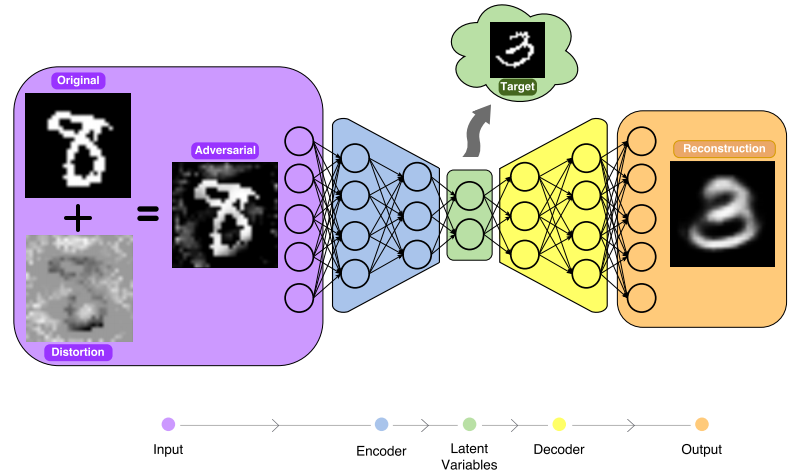
\includegraphics[width=\linewidth]{/4/adversarial_images_autoencoder}
    \caption{} 
	\label{fig:adversarial_images_autoencoder}
\end{figure}